\section{Application graphique}

\subsection{Version 0.1}

\begin{figure}[h]
\centering
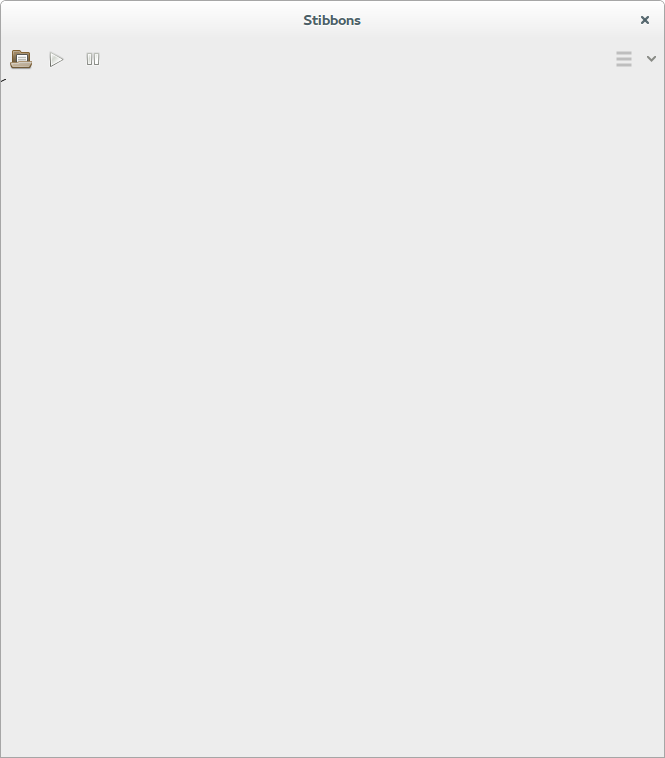
\includegraphics[scale=0.25]{doc/report/screenshot/stibbons-0-1-1.png}
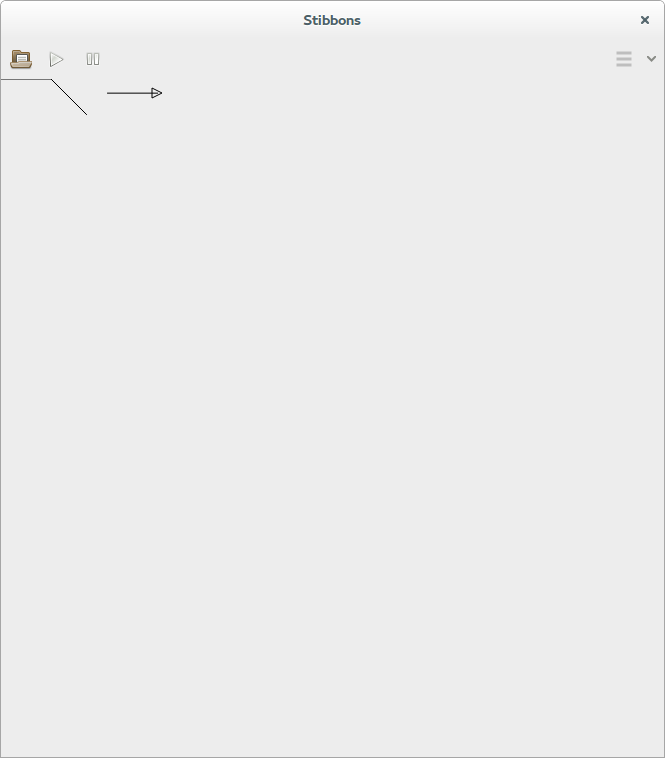
\includegraphics[scale=0.25]{doc/report/screenshot/stibbons-0-1-2.png}
\caption{\label{screenshot-0.1} Capture d'écran de la version 0.1}
\end{figure}

L'interface de la version 0.1 (cf. Figure~\ref{screenshot-0.1}) de Stibbons est composée d'une fenêtre séparée en une barre d'outil et une vue du monde.
La barre d'outil contient un bouton permettant d'ouvrir un fichier contenant un programme Stibbons (Ctrl+O), un bouton permettant d'exécuter le programme ouvert, un bouton de pause non fonctionnel, un bouton ouvrant un menu proposant la boîte de dialogues « À propos » et de quitter l'application (Ctrl+Q).

Si la boîte de dialogue permettant d'ouvrir un programme est fermée sans avoir choisi de fichier, une message d'erreur l'indiquant est alors affiché.

Une tortue existe par défaut dans le monde, elle est située dans le coin supérieur gauche de la vue et est orientée vers la droite. La tortue est alors dessinée comme un triangle noir creux et elle peut dessiner des lignes noires.

L'analyseur syntaxique n'étant à ce moment pas réentrant, ouvrir plusieurs programmes les uns après les autres implique alors de redémarrer l'application.

\subsection{Version 0.2}

\begin{figure}[h]
\centering
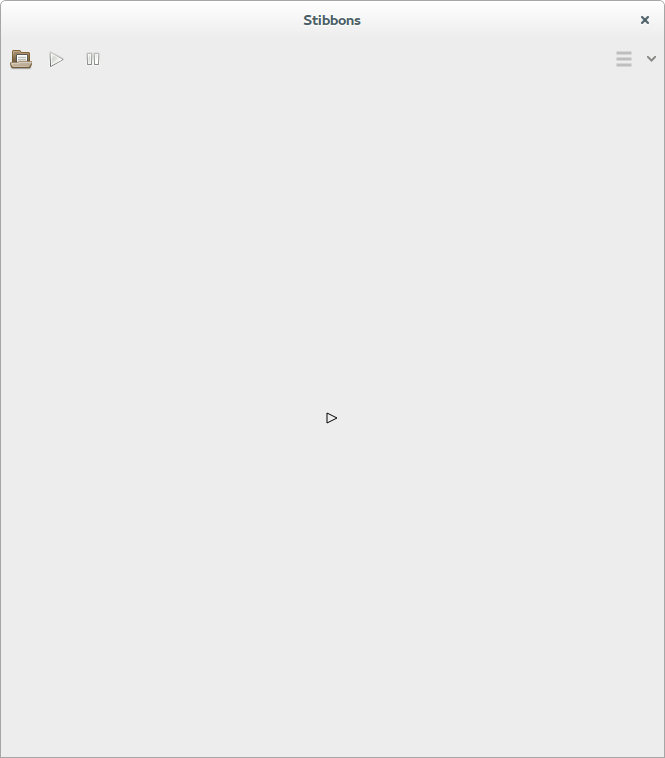
\includegraphics[scale=0.25]{doc/report/screenshot/stibbons-0-2-1.png}
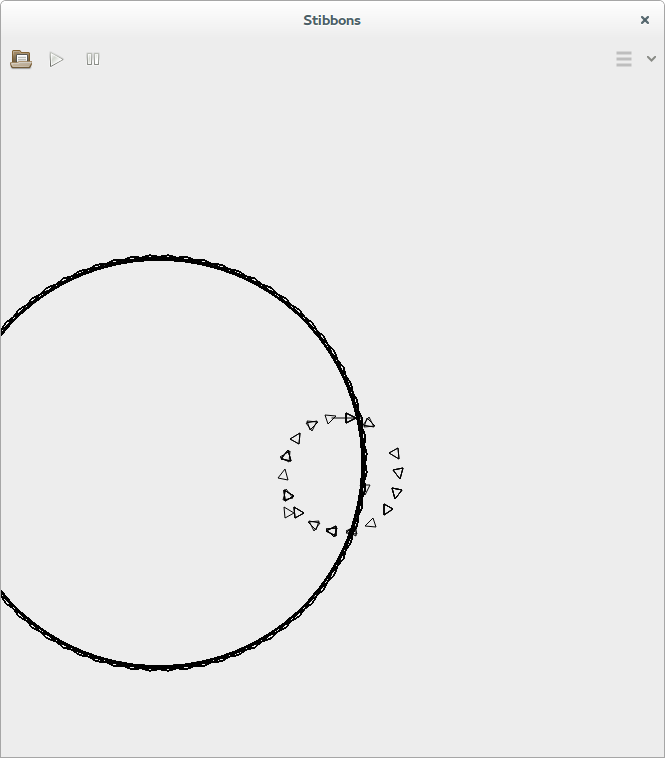
\includegraphics[scale=0.25]{doc/report/screenshot/stibbons-0-2-2.png}
\caption{\label{screenshot-0.2} Capture d'écran de la version 0.2}
\end{figure}

La version 0.2 (cf. Figure~\ref{screenshot-0.2}) apporte peu de modifications à l'application Stibbons elle-même, le changement le plus visible étant le placement temporaire de l'origine au centre de la vue, afin d'avoir une meilleure vue du programme s'exécutant.

\subsection{Version 0.3}

\begin{figure}[h]
\centering
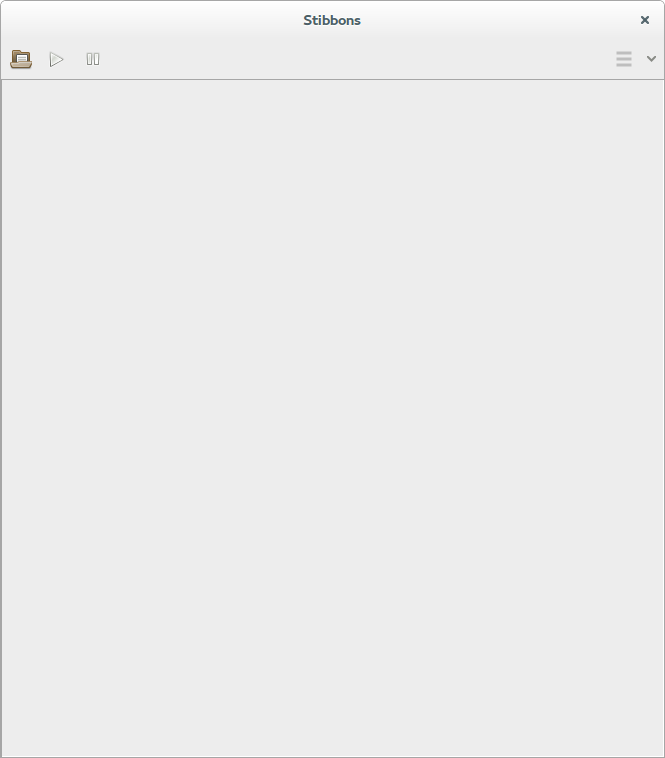
\includegraphics[scale=0.25]{doc/report/screenshot/stibbons-0-3-1.png}
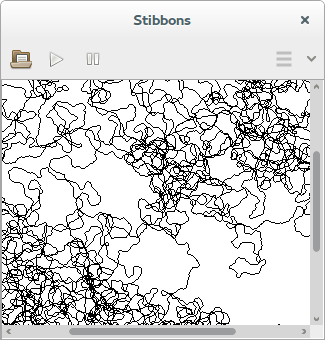
\includegraphics[scale=0.25]{doc/report/screenshot/stibbons-0-3-3.png}
\caption{\label{screenshot-0.3} Capture d'écran de la version 0.3}
\end{figure}

À partir de la version 0.3 (cf. Figure~\ref{screenshot-0.3}), les couleurs des tortues peuvent être modifiées et, afin de les rendre plus visibles, elles sont désormais dessinées comme des triangles pleins. La ligne dessinée par une tortue prend la couleur de cette dernière au moment de l'abaissement du stylo.

Le monde est désormais borné, c'est à dire que les tortues ne peuvent plus sortir du monde visible pour l'utilisateur, et est centré dans la vue, les zones le constituant sont désormais affichées, et leurs couleurs peuvent être modifiées. Si la vue est plus petite que le monde, des ascenseurs seront affichés.

Redessiner le monde prennait de plus en plus de temps au fur et à mesure que le nombre de lignes le constituant augmentait. Afin d'améliorer drastiquement ces performances de rendu, les lignes seront désormais dessinées sur un tampon et seules les nouvelles lignes auront donc besoin d'être dessinées sur ce dernier, avant qu'il soit reporté sur la vue.

\subsection{Version 0.4}

\begin{figure}[h]
\centering
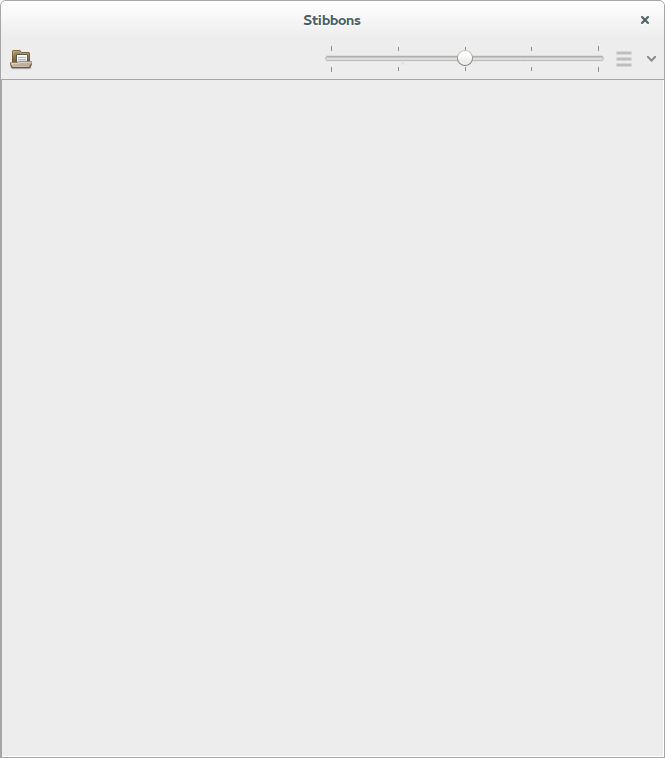
\includegraphics[scale=0.25]{doc/report/screenshot/stibbons-0-4-1.png}
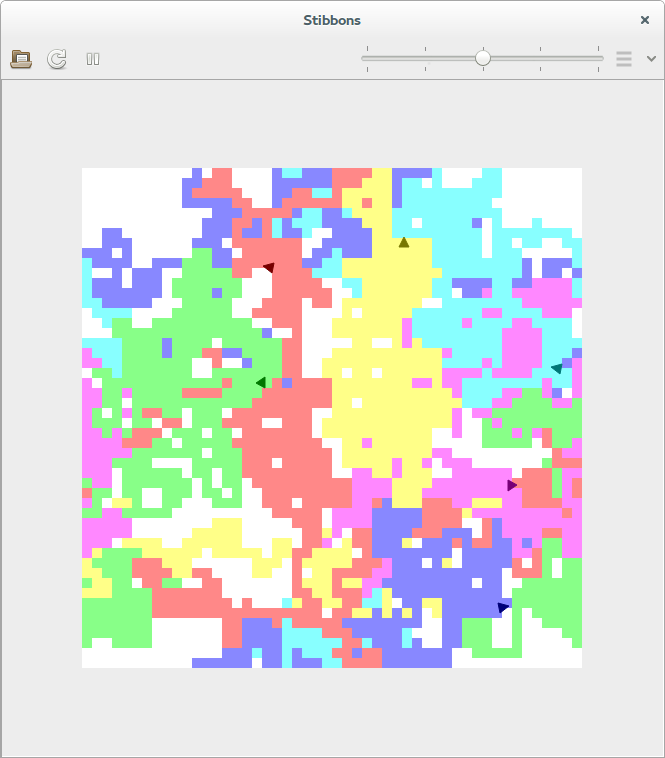
\includegraphics[scale=0.25]{doc/report/screenshot/stibbons-0-4-2.png}
\caption{\label{screenshot-0.4} Capture d'écran de la version 0.4}
\end{figure}

À partir de la version 0.4 (cf. Figure~\ref{screenshot-0.4}), il est possible de modifier la vitesse d'exécution du programme, de le mettre en pause, de reprendre son exécution et de le redémarrer depuis le début (F5). De plus, l'analyseur syntaxique étant désormais réentrant, il est possible d'ouvrir plusieurs programmes les uns à la suite des autres.

Les boutons de démarrage et de mise en pause sont désormais confondus, et sont cachés, de même que le bouton de redémarrage, tant qu'aucun programme n'a été ouvert.

Une entrée a été ajoutée au menu, permettant d'exporter le modèle en cours d'exécution.

Si une tortue change de couleur alors qu'elle trace une ligne, le stylo avec lequel la tortue trace ses lignes changera de couleur en même temps.

Il est désormais possible de faire reboucler le monde sur lui même, cette option étant paramètrable pour chaque axe. Cela permet aux tortues, lorsqu'elles atteignent un bord, d'apparaitre du coté opposé, comme si le monde était circulaire.

Le monde ne comporte plus de tortue par défaut et c'est désormais celui-ci qui exécute le corps principal du programme.

\subsection{Version 1.0}

\begin{figure}[h]
\centering
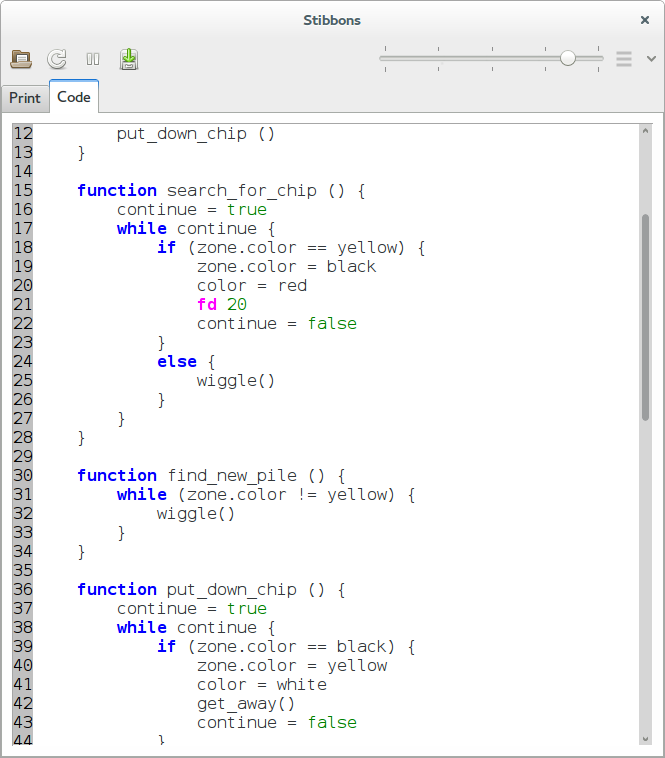
\includegraphics[scale=0.25]{doc/report/screenshot/stibbons-0-5-2.png}
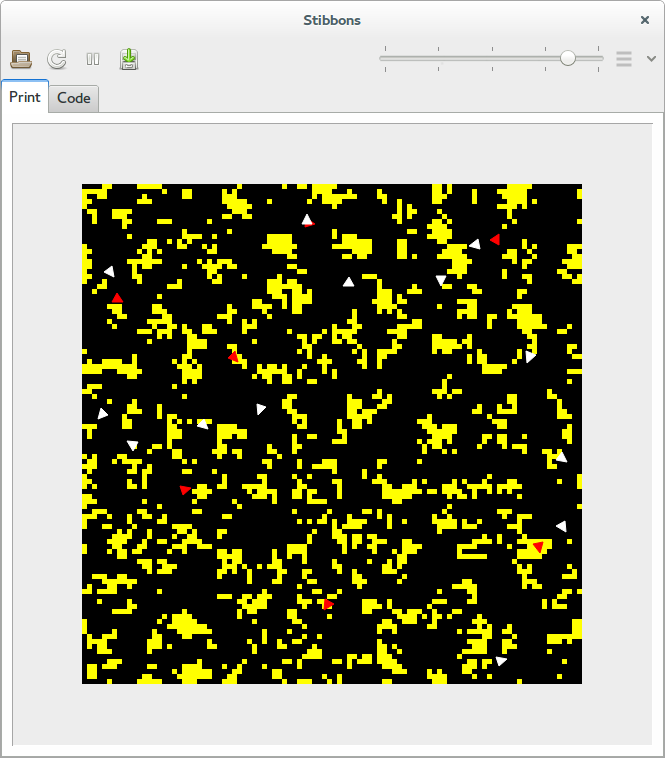
\includegraphics[scale=0.25]{doc/report/screenshot/stibbons-0-5-3.png}
\caption{\label{screenshot-1.0} Capture d'écran de la version 1.0}
\end{figure}

La version 1.0 (cf. Figure~\ref{screenshot-1.0}) marque l'apparition d'un éditeur de programme Stibbons dans l'application elle-même. L'éditeur propose également une coloration syntaxique. L'ajout de cet éditeur implique que les boutons de démarrage, de pause et de redémarrage ne soient plus cachés par défaut car il est désormais possible d'exécuter un programme écrit sans en avoir chargé un avant.

De nombreux raccourcis clavier sont ajoutés, afin d'enregistrer le programme dans son fichier (Ctrl+S) ou dans un nouveau fichier (Ctrl+Shift+S), d'exporter le modèle (Ctrl+E) et de démarrer ou mettre en pause l'exécution du programme (Ctrl+Espace).

Si la version 0.4 a ajouté une option permettant au monde de reboucler selon chaque axe, la version 1.0 permet d'avoir des bords solides, faisant rebondir toute tortue les croisant.

\section{Application en ligne de commande}

Une application en ligne de commande a été ajoutée à la version 0.4. Elle permet d'exécuter des programmes Stibbons sans serveur graphique et à pleine vitesse.

\subsection{Utilisation}

Utilisation~: stibbons-cli [options] fichier

Options~:
\begin{description}
	\item[-h, \texttt{-{}-}help] Affiche l'aide.
	\item[-v, \texttt{-{}-}version] Affiche l'information de version.
	\item[-e, \texttt{-{}-}export <secondes>] Exporte le modèle toutes les <secondes> secondes.
	\item[-p, \texttt{-{}-}prefix <prefixe>] Préfixe les fichiers exportés avec <prefixe>.
	\item[\texttt{-{}-}png] Génère une image PNG pour chaque export.
	\item[\texttt{-{}-}no-json] N'exporte pas le modèle dans un fichier JSON.
\end{description}

Arguments~:
\begin{description}
	\item[fichier] Le fichier de programme Stibbons à exécuter.
\end{description}

\subsection{Fonctionnement}

Le programme analyse la ligne de commande à l'aide de la classe \verb|QCommandLineParser|, puis crée et exécute un objet représentant l'application selon les paramètres passés par l'utilisateur.

Lors de l'exécution de l'application, il est possible d'exporter le modèle à intervalle régulier grâce à l'option \verb|--export|. Par défaut, le modèle est exporté dans un fichier JSON, mais il est également possible d'exporter un rendu du monde en PNG, ou encore de ne rien exporter.

Afin de pouvoir dessiner le monde dans un fichier image, la classe \verb|WorldView|, widget de l'application graphique jusque là responsable de dessiner le monde sur lui même, a vu ses fonctionnnalités de dessin d'un monde migrer vers la nouvelle classe \verb|WorldPainter|, capable de dessiner un monde sur une surface.
Cette nouvelle classe est désormais utilisée dans l'application graphique par \verb|WorldView| pour se dessiner, et par l'application en ligne de commande pour dessiner sur une \verb|QImage|.
